\documentclass[journal=jpcafh,manuscript=article,layout=onecolumn, 12pt]{achemso}
\usepackage[version=3]{mhchem} % Formula subscripts using \ce{}
\usepackage[T1]{fontenc}       % Use modern font encodings
\usepackage{amsmath}
\usepackage[dvipsnames]{xcolor}
% NB added command for in line cite
\newcommand{\onlinecite}[1]{\hspace{-1 ex} \nocite{#1}\citenum{#1}} 
%
\author{Benjamin~A.~Laws}
\email{b.laws@unsw.edu.au}
\affiliation{School of Chemistry, University of New South Wales, Sydney NSW 2052, Australia}
\alsoaffiliation{Research School of Physics, The Australian
	National University, Canberra ACT 2601, Australia}
\author{Zachariah~D.~Levey} 
\affiliation{School of Chemistry, University of New South Wales, Sydney NSW 2052, Australia}
\author{John F. Stanton}
\affiliation{Department of Chemistry, University of Florida, Gainesville, Florida 32611, United States}
\author{Timothy~W.~Schmidt} 
\affiliation{School of Chemistry, University of New South Wales, Sydney NSW 2052, Australia}
\author{Stephen~T.~Gibson}
\affiliation{Research School of Physics, The Australian
	National University, Canberra ACT 2601, Australia}
\title{Vibronic coupling in C$_2$H: implications for astrochemistry}
\abbreviations{PES,PAD,EA,eKE,FWHM,VMI}
\begin{document} 
\begin{abstract} 

\end{abstract}
\section{Introduction}
Carbon monohydrides C$_{2n}$H, are a class of linear radicals that play an important role in combustion and interstellar chemistry. These carbon chains have been observed in many interstellar environments, including planetary atmospheres, comets, dark clouds, and during heavy star formation. Due to their relatively high abundance in a variety of astronomical conditions, they are believed to be promising candidates for Diffuse Interstellar Band (DIB) carriers. The corresponding anions C$_{2n}$H$^-$ are also believed to play an important role in interstellar chemistry. C$_6$H$^-$ was the first negative ion detected in space, after it was observed in two distinct interstellar molecular clouds IRC+10216 and TMC-1 in 2006. More recently, anions C$_4$H$^-$ and C$_8$H$^-$ have also been detected in a range of environments, include dark clouds, prestellar cores, and prostellar envelopes.

Chain growth of the C$_{2n}$H radicals occurs predominately through acetylene addition,
\begin{equation}
\text{C}_{2n}\text{H} + \text{C}_2\text{H}_2 \rightarrow \text{C}_{2n+2}\text{H}+\text{H}_2.
\end{equation}
Conversely, the formation of anions in space is believed to be driven by radiative electron attachment, charge transfer, and dissociate electron attachment. Current astrochemical modelling of interstellar clouds, such as IRC+1026, typically underestimate the observed abundances of CH$_4^-$. Therefore, it has been proposed that ion-neutral reactions
 \begin{equation}
	\text{C}_{2n}\text{H}^- + \text{C}_2\text{H}_2 \rightarrow \text{C}_{2n+2}\text{H}^- + \text{H}_2.
\end{equation}
may be significant chain growth mechanisms that also needs to be included. Modelling of the extraterrestrial planetary atmosphere of Saturn's moon Titan, suggests that both C$_2$H and C$_2$H$^-$ play an important role in the atmospheric chemistry. Multiple reaction pathways were included for the ion C$_2$H$^-$ including reactions with C$_2$H$_2$ and HCN. 

Understanding interstellar chemistry relies critically on theory, to provide a link between astronomical observations and terrestrial laboratory studies. Microwave spectroscopy has successfully been used in this fashion to identify a large number of molecules in the interstellar medium (ISM). However for some species, particularly those with low abundances or no dipole moment, UV/vis spectroscopic methods are required for identification. This creates a challenge for theory, as electronic spectra calculations are more sensitive to the level of theory employed than pure rotational spectra. This becomes even more challenging when vibronic coupling effects are introduced, as they can be exceedingly difficult to model.

These considerations may be explored by examining some of the smallest carbon monohydrides. The ethynyl radical C$_2$H may appear to be a simple linear triatomic molecule. However the electronic spectrum is complicated by the presence of the close-lying ground $^2\Sigma^+$ and first excited $^2\Pi$ surfaces, which are only separated by $\sim3,600~$cm$^{-1}$. The interaction of these surfaces produces a complex vibronic spectrum around the $\tilde{A}^2\Pi$ state, where the $\tilde{X}-\tilde{A}$ origin is spread over multiple admixed vibronic levels. In C$_4$H the $^2\Sigma^+$ and $^2\Pi$ states are nearly degenerate, resulting in even stronger coupling, while in C$_6$H and C$_8$H the ordering of the states swaps, with a ground $^2\Pi$ state and a low lying excited $^2\Sigma^+$ state. Consequently, understanding these vibronic coupling interactions between the $^2\Sigma$ and $^2\Pi$ surfaces will be essential in order to accurately model the role these radicals (and their corresponding anions) are likely to play in the interstellar chemistry mentioned above, and to guide the search for possible DIB carriers.

In this paper we study the vibronic spectrum of the ethynyl radical C$_2$H by employing High-Resolution Photoelectron Imaging (HR-PEI) in order to benchmark CFOUR \emph{ab-initio} vibronic-coupling calculations. C$_2$H is reported to be one of the most abundant molecules in the universe, and is the most thoroughly studied of the C$_{2n}$H species. Many different experimental techniques have been employed to try and resolve the complex vibronic spectrum, including electron spin resonance, laser magnetic resonance, microwave and milli-meter wave spectroscopy, infrared (matrix isolation and Fourier Transform) spectroscopy, and photoelectron spectroscopy. C$_2$H has also received extensive theoretical attention to try and understand the experimental results, however the large number of possible vibronic levels means this has proven to be a challenge. In this work we demonstrate how construction of a quasiadiabatic Hamiltonian allows for the strength of vibronic interactions between coupled surfaces near a conical intersection to be calculated, in order to simulate electronic and vibronic spectra. By employing anion HR-PEI both the $^2\Sigma^+$ and $^2\Pi$ surfaces are mapped out on an equal footing from the anion $\tilde{X}^1\Sigma^+$ state, allowing for direct comparison to the \emph{ab-initio} modelling.

\section{Results and Analysis}
Ethynyl ions were produced in a pulsed-jet discharge of pure C$_2$H$_4$ gas, and subsequently mass isolated via time of flight. Electrons were detached using a tuneable Sunlite Optical Parametric Oscillator (OPO) pumped with the third harmonic of a Nd:YAG laser. High electron counts could also be obtained by using the third and fourth harmonics of the Nd:YAG laser directly. The detached electrons were then mapped onto a micro channel plate detector using a Velocity Map Imaging (VMI) lens. An illustrative VMI of $\sim$4 million electrons collected from 355~nm (3.49~eV) photodetachment of C$_2$H$^-$ is shown in Fig.~\ref{fig:1}(a). The electrons are distributed radially according to their speed, with slow electrons at the image center, and fast electrons located towards the outer edge. Due to the relatively large C$_2$H$^-$ electron affinity (EA) of 2.969~eV~\cite{erv91}, photodetachment at 355~nm occurs close to threshold. This yields slow electrons, allowing for a low repeller voltage ($-600$~V) on the VMI lens, and high velocity resolution. 


Despite being close to threshold, two electronic states of neutral C$_2$H are observed. The faster electrons on the outer edge correspond to C$_2$H$(\tilde{X}\,^2\Sigma^+)+e^- \leftarrow $C$_2$H$^-(\tilde{X}\,^1\Sigma^+)+h\nu$ photodetachment, and are preferentially distributed around the poles of the image, indicative of a positive anisotropy parameter. Conversely the angular distribution of the slower electrons near the center are skewed towards the equator, indicative of a negative anisotropy parameter. These electrons may be assigned to photodetachment to the first excited state C$_2$H$(\tilde{A}\,^2\Pi)+e^- \leftarrow $C$_2$H$^-(\tilde{X}\,^1\Sigma^+)+h\nu$.

\begin{figure}
	
\includegraphics[width=0.8\textwidth]{figures/Fig1}
	\caption{(a) A 3D-representation of the velocity-map image of $\sim$ 4 million photoelectrons detached from C$2$H$^-$ at 355~nm. The outer rings, distributed around the vertical laser polarisation axis, represents photodetachment to the ground $\tilde{X}\,^2\Sigma^+$ state. The inner rings reprsent detachment to the first excited state $\tilde{A}\,^2\Pi$. (b) Photoelectron spectra of C$_2$H$^-$ at a range of detachment wavelengths, illustrating the change in electron intensity profile and energy resolution.}
	\label{fig:1}
\end{figure}

To investigate the vibronic coupling interaction between these two nearby $\Sigma^+$ and $\Pi$ surfaces, deuterated ethynyl C$_2$D$^-$ was also studied. C$_2$D$^-$ ions were produced in a discharge of pure C$_2$D$_4$ gas and measured under the same experimental conditions as C$_2$H$^-$. An illustrative VMI of photodetachment at 355~nm from C$_2$D$^-$ is shown in Fig.~\ref{fig:1}(b). Similarly to Fig~\ref{fig:1}(a) two electronic transitions are observed. While the fast electrons appear similar in both images, a striking difference is observed in the slow electrons near the detector center. In Fig.~\ref{fig:1}(a) a series of weak rings are observed, however in Fig.~\ref{fig:1}(b) two dominant rings are seen.

The VMIs in Fig.~\ref{fig:1} were inverted using the Abel inversion methods detailed in pyAbel, to extract the corresponding photoelectron spectra presented in Fig.~\ref{fig:1}(c). Below $27,000~$cm$^{-1}$ on the $\tilde{X} ^2\Sigma^+$ surface the C$_2$H$^-$ and C$_2$D$^-$ spectra are very similar. Both are dominated by the origin transition, shifted by $\sim10~$cm$^{-1}$ in the deuterated spectrum, with progressions involving the v$_2$($\pi$) bending and v$_3$($\sigma$) CC stretch vibrational normal modes. This includes transitions involving an odd quanta of v$_2$ bending excitation ($2^{n+1}$) which should be totally forbidden within the harmonic oscillator approximation. However, the presence of these transitions in the spectra is likely an indicator of Herzberg-Teller (HT) vibronic coupling between the ground $^2\Sigma^+$ and nearby excited $^2\Pi$ electronic surfaces, as
\begin{equation}
\Sigma^+ \otimes \pi = \Pi. 
\end{equation}

Above $27,000~$cm$^{-1}$, near the $\tilde{A}^2\Pi$ state origin, large differences are observed between the C$_2$H$^-$ and C$_2$D$^-$ photoelectron spectra. In the C$_2$H$^-$ spectrum 5 sharp peaks are observed, spaced by $\sim95~$cm$^{-1}$. However in the deuterated spectrum, one dominant peak is observed at $27,792$~cm$^{-1}$, with 3 weaker peaks centred around $27,360~$cm$^{-1}$. Unlike the structure below $27,000$~cm$^{-1}$ none of these peaks are able to be readily assigned to vibronic transitions, due to the presence of strong coupling interactions between the nearby $\Sigma^+$ and $\Pi$ surfaces.




\subsection{Vibronic Coupling Interactions}
The complex spectral structure observed near the $\tilde{A}^2\Pi$ state origin in Fig.~\ref{fig:1}(c) may be understood by considering the $v_2$ bending vibrational mode. To account for the degeneracy of this mode, the vibronic quantum number $\ell_i$ may be introduced, representing the angular momentum associated with the bending motion. This may take a value of $\ell_i = v_i, v_i-2, v_i-4,\dots,1$ or $0$, where $v_i$ is the quanta of bending excitation. In the Born-Oppenheimer approximation different vibronic energy levels $\ell_i$ are degenerate, however in cases with strong rovibronic coupling, this degeneracy in $\ell_i$ is lost. 

In C$_2$H this effect creates a Renner-Teller (RT) pair in the excited state, where the usually degenerate $\Pi$ surfaces separate to form two non-degenerate electronic states $\Pi^+ (2A')$ and $\Pi^-(1A'')$. This involves separating a single potential energy surface (V) into two distinct but connected surfaces (V$^+$) and (V$^-$). Due to the strong coupling along the linear axis between the electronic and vibration angular momenta of the $2A'$ and $1A''$ components of the $^2\Pi$ state, stationary states cannot be explicitly assigned to either of the $\Pi^+(2A')$ or $\Pi^-(1A'')$ electronic surfaces. Instead, they exist as a combination of both states.

Due to the close lying nature of the ground {$\tilde{X} ^2\Sigma^+$} and excited {$\tilde{A} ^2\Pi$} electronic states, which are only separated by $\sim3700~$cm$^{-1}$, a pseudo Jahn-Teller effect is also observed. %The Jahn-Teller theorem states that stability and degeneracy are not possible simultaneously unless the molecule is linear~\cite{jah37}, meaning that non-linear molecules with degenerate electronic states will undergo a symmetry breaking distortion in order to remove the degeneracy. However a similar effect has also been observed where coupling exists between a non-degenerate state and a nearby pair of degenerate states, even if a molecule is linear. 
In the case of C$_2$H this is seen as coupling between the ground $\Sigma^+(1A')$ and excited $\Pi^+(2A')$ states, induced by the bending motion of $v_2$. The ground state only couples to one of the Renner-Teller pair $\Pi^+(2A')$, as the other state $\Pi^-(1A'')$ has incorrect symmetry. This results in the complex vibronic structure observed for the $\tilde{A}^2\Pi$ electronic state, with contributions from three coupled surfaces $\Sigma^+(1A'),$ $\Pi^+(2A'),$ and $\Pi^-(1A'')$.

These interactions spread the electronic orgin of the $\tilde{A}\,^2\Pi$ state over several vibronic levels. Therefore, instead of assigning a defined origin, the observed peaks in the spectrum may be assigned to coupled admixtures of vibronic transitions involving the three potential energy surfaces,
\begin{equation}
\Psi_f = \sum_\xi \psi_e^\xi \sum_k C_{fk}^\xi\phi_{fkm}^\xi,
\label{eq:teller3} 
\end{equation}
where $\psi_e^\xi$ is the diabatic electronic wavefunction, and $\phi_{fkm}^\xi$ is the spin-rovibrational wavefunction. $\xi$ represents the electronic states used in the expansion ($\xi=\Sigma^+(1A'),~\Pi^+(2A'),~\Pi^-(1A'')$). A depiction of these three interacting surfaces is given in Fig.~\ref{fig:3}.

\begin{figure}
	\centering
	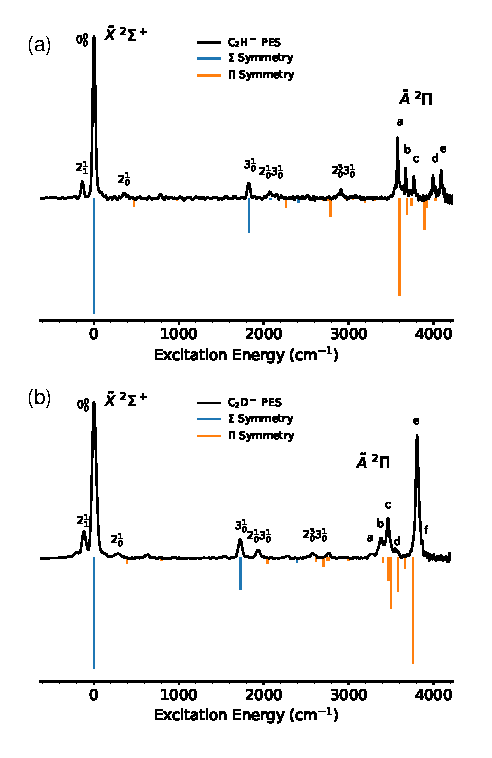
\includegraphics[width=0.5\textwidth]{figures/Fig3}
	\caption{Adiabatic potential energy surfaces of $\tilde{X}^2\Sigma^+$, $\tilde{A}^2\Pi^-$, and $\tilde{A}^2\Pi^+$ states, calculated using the method developed by Tarroni and Carter~\cite{tar03} (E$_{1A'}$, E$_{2A'}$, and E$_{1A''}$ in Eq.~\ref{eq:teller3}).}
	\label{fig:3}
\end{figure}

The adiabatic potential energy surfaces in Figure~\ref{fig:3} were calculated using the variational method of Tarroni and Carter. This has been used to calculate a multitude of admixed vibronic levels. In the literature, over 100 possible C$_2$H vibronic states have been calculated, up to 6,400~cm$^{-1}$ above the $\tilde{X} ^2\Sigma^+$ origin. However, assigning experimental spectra has remained a challenge, partly due to the large number of calculated levels providing multiple possible assignments for each experimentally observed transition.


\subsection{Coupling Calculations}
In order to guide spectral assignment of C$_2$H and astronomical searches for other C$_n$H radicals, transition intensities are also needed. However, due to the strong vibronic coupling interactions, this can not be obtained via standard quantum chemistry methods. To account for these interactions, the photoelectron spectrum of the C$_2$H$^-$ anion was simulated using a quasidiabatic Hamiltonian of the type advocated by Koeppel, Domcke and Cederbaum (KDC, reference here).   In this approach, the Hamiltonian is represented in a basis of quasidiabatic (slowly varying) electronic  states for which the kinetic energy operator can be assumed diagonal.   For C$_2$H, the KDC Hamiltonian comprises three states - the two components of the $^2\Pi$ state and the ground $^2\Sigma$ state - and is then projected onto a vibrational basis, usually chosen as a direct product of harmonic oscillators.  Diagonalization of the corresponding matrix yields the molecular states (which are given in terms of a Born-Huang expansion), and the squared projections of the corresponding eigenvectors onto the ground state of the anion yield the relative intensities. The latter is automatically true if the photodetachment cross sections for the $^2\Sigma$ and $^2\Pi$ states are assumed equal, but different cross sections of the two states can be incorporated by scaling the intensities of states according to their (vibronic) symmetry. 

Details of the construction and parametrization of KDC Hamiltonians can be found elsewhere in the literature (references), and the procedure followed will be discussed here only briefly.   The present calculations use the so-called quadratic vibronic coupling (QVC) model.  For the system at hand, the QVC model Hamiltonian  assumes the following form

\begin{align}
H &= T_n1+V\\
V &= \bordermatrix{ & X & A(a') & A(a'') \cr
	X &\substack{\Delta_0^X+F_1^Xq_1+F_3^Xq_3+\\ 
		\frac{1}{2} \sum_{ij}F^X_{ij}q_iq_j}& \lambda q_{2a} & \lambda q_{2b} \cr
	A(a') & \lambda q_{2a} & \substack{\Delta^A_0+F^A_1q_1+F^A_3q_3\\+\frac{1}{2}\sum_{ij}F^A_{ij}q_iq_j+\\\frac{1}{2}\eta(q_{2a}^2-q_{2b}^2)} & \eta q_{2a}q_{2b} \cr
	A(a'') & \lambda q_{2b} & \eta q_{2a}q_{2b} & \substack{\Delta_0^A+F_1^Aq_1+F_3^Aq_3\\+\frac{1}{2}\sum_{ij}F_{ij}^Aq_iq_j\\-\frac{1}{2}\eta(q_{2a}^2-q_{2b}^2) } } \qquad
\label{eq:calc1}
\end{align}

where the summations run over the dimensionless normal modes ($q_i$) that serve as the coordinate system for the problem.   For convenience, the latter are chosen to be those of the anion, which considerably facilitates calculation of the spectral intensities.  In Eq.~(\ref{eq:calc1}), the diagonal terms of V (excluding those that carry the Renner-Teller coupling constant $\eta$) represent the quasidiabatic potential energy surfaces of the $\Sigma$, and the two components of the $\Pi$ state, chosen here as those in which the unpaired electron lies within or is perpendicular to an arbitrarily chosen plane, designated as A(a$'$) and A(a$''$), respectively. $\Delta_0^X$ is the separation of the anion and $\Sigma$ states at the origin of the coordinate system (the vertical electron detachment energy), and $\Delta_0^{A}$ is the gap between anion and $\Pi$ states at the same geometry.   

For the modes of $\sigma$ symmetry ($q_1$ and $q_3$), the diabatic forces ($F_i$) and force constants ($F_{ij}$) coincide with those of the adiabatic potential energy surfaces.   However, for the bending mode, the diabatic (F$_{22}$) and adiabatic (f$_{22}$) force constants differ, and the parametrization is somewhat more involved.   For each component of the $\Pi$ state, either the 2a or 2b component of the bending vibration will maintain the A$'$ electronic symmetry that is needed to couple with the X state.  Designating these as 2a for the A(a$'$) state and 2b for the A(a$''$) state (as is implicit in Eq.~\ref{eq:calc1}), the diabatic force constants for the bending mode in the X and A states can be written as 

\begin{align}
F_{22}^X &= f_{22}^X+\frac{2\lambda^2}{(\Delta_0^A-\Delta_0^X)}\\
F_{22}^A &= f_{2a2a}^{A(a')}-\frac{2\lambda^2}{(\Delta_0^A-\Delta_0^X)}-\eta
\label{eq:calc2}
\end{align}

where the Renner-Teller interaction strength ($\eta$) is determined from 

\begin{equation}
\eta = \frac{1}{2}\left[ f_{2a2a}^{A(a')}-f_{2b2b}^{A(a')}-\frac{2\lambda^2}{(\Delta_0^A-\Delta_0^X)}\right]
\label{eq:calc3}
\end{equation}

once the interstate coupling ($\lambda$ which is calculated analytically in this work, see below) is known.

When the potential in Eq. 1 is diagonalized, the adiabatic states that are used for its parametrization are precisely recovered through second order in displacement. To parametrize this Hamiltonian, the equation-of-motion coupled-cluster method known as EOMIP-CCSDT has been used to optimise the geometry of the ground state anion, with an Atomic Natural Orbital (ANO) basis (ANO2). Adiabatic linear and quadratic force constants are calculated from the analytical derivatives of the \emph{ab-initio} potential energy surface with respect to the anion reduced normal coordinates, at the anion geometry Q$_0$. The interstate PJT coupling constant $\lambda$ is evaluated directly using the CFOUR package to employ the quasidiabatic ansatz described in refs. This allows for direct ab-initio evaluation of the linear diabatic interstate coupling constants that parametrize the KDC potential. The calculated parameters are presented in the Supplementary Materials, in Table S1.   



\subsection{Simulated Spectra}
The above method was employed to simulate the photoelectron spectrum of C$_2$H$^-$, with the calculated transitions shown in Figure~\ref{fig:C2H-plot}(a) alongside the experimental data at 355~nm. %Calculated transitions with $\Sigma$ symmetry are in blue, and transitions with $\Pi$ symmetry are in orange. 
On the $\tilde{X} ^2\Sigma^+$ surface, below 3,600~cm$^{-1}$, there is excellent agreement in both the transition positions and intensities between the simulated and experimental spectra. This includes the HT coupled (2$^{n+1}$) transitions with $\Pi$ symmetry, which would normally be missing from a simulation using standard \emph{ab-initio} approaches. 

The positions of the calculated levels for the $\tilde{A}^2\Pi$ state have been shifted by 1,220~cm$^{-1}$ to account for the EOMIP-CCSDT calculations overestimating the effective Term energy. The experimental data shows that the electronic coupling interactions induce a splitting of the $\tilde{A} ^2\Pi$ state origin over 5 vibronic levels, spaced by $\sim 95~$cm$^{-1}$ (a-e). This splitting is also observed in the calculated spectrum, which correctly predicts 5 prominent transitions in this region. The relative intensities between the calculated transitions are also in good agreement with the experimental data. Peak d is slightly underestimated, however the relative intensity difference between peaks d and e may be partly explained by the Wigner threshold law, which will reduce the intensity of peak e in the experimental spectrum as it is close to the detachment threshold. The simulated spectrum also slightly underestimates the splitting between the vibronic levels, which may be linked to the overestimation of the gap between the $^2\Sigma$ and $^2\Pi$ surfaces.

\begin{figure}[th!]
	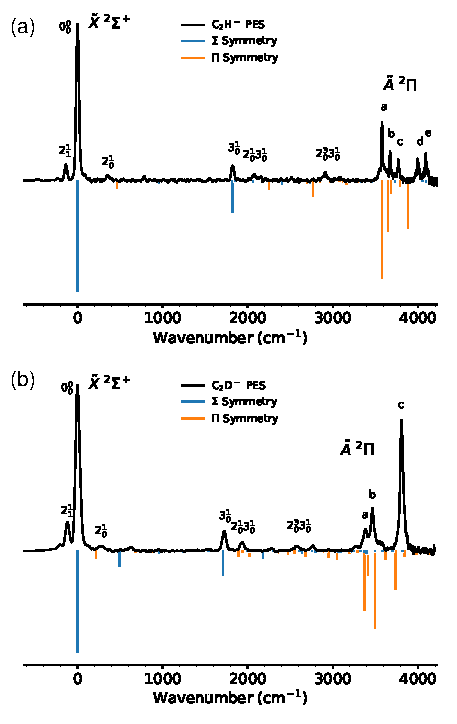
\includegraphics[width=0.6\textwidth]{figures/Fig5.pdf}
	\caption{cat}
	\label{fig:C2H-plot}
\end{figure}

The photoelectron spectrum of C$_2$D$^-$ was also examined using the same approach, with the calculated transitions shown in Figure~\ref{fig:C2H-plot}(b) alongside the 355~nm experimental data. Again, there is excellent agreement in the intensity and calculated positions of the transitions on the $\tilde{X} ^2\Sigma^+$ state surface, including the HT coupled levels. Near the $\tilde{A} ^2\Pi$ state origin, deuteration has a large impact on the experimental photoelectron spectrum. Instead of the 5 evenly split levels observed in C$_2$H, a single dominant peak (d) is now observed at 3,844~cm$^{-1}$ alongside a collection of weaker peaks (a-c) centred around 3,400~cm$^{-1}$. Based on previous spin-orbit splitting measurements, peak d is expected to have significant $\tilde{A} ^2\Pi$ character, with peaks a-c commonly assigned to vibronic levels with predominantly HT coupled $\tilde{X} ^2\Sigma^+$ character. This suggests that deuteration effectively dampens the coupling interaction between the surfaces.

Like the experimental spectra, a large change is observed in the simulated spectrum upon deuteration. The calculated intensity pattern of the vibronic levels around the $\tilde{A} ^2\Pi$ origin is a good match to the experimental data, with a single intense transition observed near peak d, and 3 prominent transitions predicted around the experimental peaks a-c. The calculated splitting between the levels is also similar, however the relative intensity of peak d appears to be slightly underestimated. %The results from Figure~\ref{fig:C2H-plot} confirm that the quasiadiabtic approach is able to accurately describe the vibronic interactions between the $\Sigma$ and $\Pi$ surfaces, including deuteration effects.      

\begin{figure}[th!]
	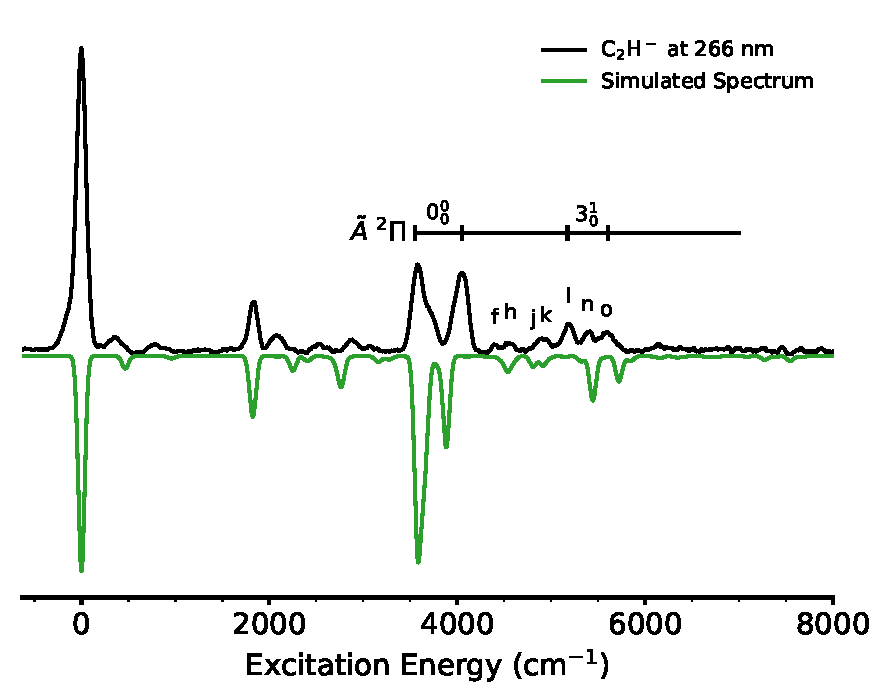
\includegraphics[width=0.6\textwidth]{figures/266-plot.pdf}
	\caption{cat}
	\label{fig:266-plot}
\end{figure}
To investigate the effects of coupling on the higher excited vibronic levels on the$\tilde{A} ^2\Pi$ surface, the calculations were compared to the experimental photoelectron spectrum of C$_2$H$^-$ at 266~nm, as presented in Figure~\ref{fig:266-plot}. Gaussians were fitted to the transitions from Figure~\ref{fig:C2H-plot}(a) with a FWHM of 40~cm$^{-1}$ to match the resolution of the experimental data above threshold. Near 3,900~cm$^{-1}$ the electronic origin of the $\tilde{A} ^2\Pi$ state is split over 5 vibronic levels, as discussed above. A similar effect is also observed for the $3^1_0$ band, which becomes split over 3 vibronic levels labelled l, n, and o. The calculated spectrum correctly predicts the position and intensity of peaks n and o, but appears to strongly underestimate the intensity of peak l. Between the $0^0_0$ and $3^1_0$ bands a collection of weaker peaks are also observed (f,g,j,k). These are assigned to highly excited HT coupled $\tilde{X} ^2\Sigma^+$ transitions (j,k), and pure $\tilde{X} ^2\Sigma^+$ transitions (f,g). Consequently, peaks f and g will possess $\Sigma$ symmetry, and should have a different anisotropy to all of the other dominant transitions above 3,800~cm$^{-1}$. The position and intensity of these highly-excited coupled transitions are well described by the simulated spectrum. 

The results from Figures~\ref{fig:C2H-plot} and~\ref{fig:266-plot} confirm that the quasiadiabtic approach is able to accurately describe the vibronic interactions between the $\Sigma$ and $\Pi$ surfaces, including deuteration effects. This validates the proposed vibronic interactions, and demonstrates how this method can be employed to decode and assign even complex spectra. Applying this approach to similar less-studied systems will produce reliable predictions for the position and intensity of dominant transitions, which will help guide the search for these molecules in laboratory experiments and astronomical observations. 



%Overall, figures a-c show that the quasiadiabatic approach is a reliable method for simulating the spectra of molecules when strong vibornic coupling interactions are involved. This method may be expanded to other C$_n$H radicals that possess similar complexities, in order to help guide the search for new molecules to be found in space.

\subsection{Photoelectron Angular Distributions}
Symmetry considerations may be employed to verify the spectral assignments from the calculations above. The quasiadiabatic Hamiltonian approach is able to determine the symmetry of each individual vibronic state, either $\Sigma$ or $\Pi$, which may be compared directly to the experimental electron anisotropy of each transition. The VMIs from this work (Figure~\ref{fig:1}) were obtained using a linearly polarized detachment laser. Therefore, the differential cross section of emitted electrons is given by  
\begin{equation}
	\frac{\text{d}\sigma}{\text{d}\Omega}=\frac{\sigma_{\text{total}}}{4\pi}[1+\beta P_{2}(\cos\theta)],
	\label{eq:beta1}
\end{equation}
where $\theta$ is the angle between the ejected electron and the (vertical) 
laser polarization, and $P_2$ is the second-order Legendre polynomial. The anisotropy parameter $\beta$ provides a quantitative measure of the anisotropy, and can range from -1 to +2 for purely perpendicular and parallel transition respectively. Through conservation of angular momentum, $\beta$ may be described in terms of the detachment partial waves, which are linked to the symmetry of the parent detachment orbital. This is discussed in detail elsewhere [cite], and will be only briefly described for the case of C$_2$H$^-$ here. 

Photodetachment to the ground state of C$_2$H$^-$ $(\tilde{X}\,^1\Sigma^+)$ involves ejecting an electron from an $s-$like $5\sigma_g$ orbital, whereas detachment to the excited $(\tilde{A}\,^2\Pi)$ state occurs from a $p-$like $1\pi_u$ orbital. Therefore, the electron anisotropies may be described using the mixed $sp$ model,
\begin{equation}
\beta(\epsilon)_{sp} = \frac{2Z\epsilon+2\text{A}_1\epsilon^2-4\epsilon\cos\delta_{\ell\pm 1}}{\frac{1}{\text{A}_1}+2\text{A}_1\epsilon^2+Z\epsilon}
\label{eq:beta-sanov}
\end{equation}  
where $\epsilon$ is the electron kinetic energy, $A_1$ is the $s\rightarrow p$ Hanstorp coefficient, $f$ is the percentage of $p$ orbital character,
\begin{equation}
Z = \frac{1-f}{f}\frac{8}{3}~~ \text{and} ~~ |\psi\rangle = \sqrt{1-f}|s\rangle + \sqrt{f}|p\rangle.
\end{equation}

From Eq.~(\ref{eq:beta-sanov}) it can be seen that detachment from a pure $s$ orbital will have a positive anisotropy ($\beta=+2$), whereas detachment from a pure $p$ orbital will have a negative anisotropy for electron kinetic energies $\epsilon < 2/A_1$. Therefore, measuring the anisotropy will determine the electronic character of each individual transition, which may be compared to the calculated symmetries in Figure~\ref{fig:C2H-plot}. The anisotropy parameters were measured for every detachment wavelength and prominent transition in the C$_2$H$^-$ photoelectron spectra from this work, and are presented in Figure~S1. Fitting Eq.~(\ref{eq:beta-sanov}) to the $^2\Pi$ state detachment with f=0.9 produces a Hanstorp coefficient of $A_1$=0.66(4)~eV$^{-1}$. 

\begin{figure}[th!]
	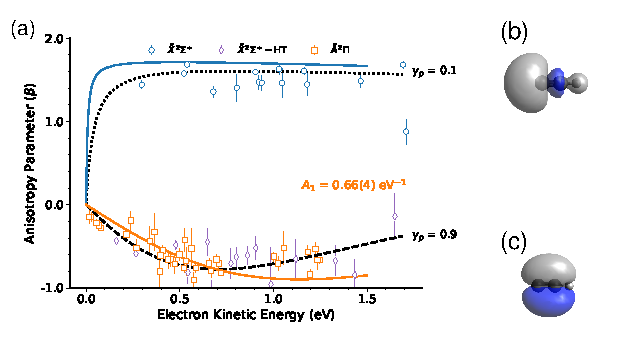
\includegraphics[width=0.5\textwidth]{figures/PAD.pdf}
	\caption{cat}
	\label{fig:S1}
\end{figure}

The sign (+/-) of $\beta$ can be used to assign each vibronic level to either the $^2\Sigma^+$ $\leftarrow^1\Sigma^+$ or $^2\Pi$ $\leftarrow^1\Sigma^+$ electronic transition respectively. This is particularly useful around the $\tilde{A} ^2\Pi$ origin, where the two states overlap. It is important to note that the HT coupled transitions on the $\tilde{X} ^2\Sigma^+$ surface have negative anisotropies and $\Pi$ symmetry. This is discussed in more detail in the Supplementary Materials.

A plot of the anisotropy parameters for C$_2$H$^-$ detachment at 300~nm is presented in Figure~\ref{fig:beta}, alongside the experimental spectrum. By plotting $\beta\times I$ the sign (+/-) of each individual transition can be easily identified. All of the transitions above the $\tilde{A} ^2\Pi$ origin have a negative anisotropy, except for peak f. This confirms the assignment of this peak to the highly excited $\Sigma$ transition $\tilde{X}(0,6,1$). The nearby peak h is assigned to the admixed $\Pi$ transition $\tilde{X}(0,3,2)\tilde{A}(0,0,0)$. The other two peaks in this region j and k are assigned to highly excited HT coupled $\Pi$ transitions $\tilde{X}(0,7,1)$ and $\tilde{X}(0,11,0)$. The assignments for all peaks in the C$_2$H$^-$ and C$_2$D$^-$ photoelectron spectra are presented in the Supplementary Materials Table~S1.

\begin{figure}[th!]
	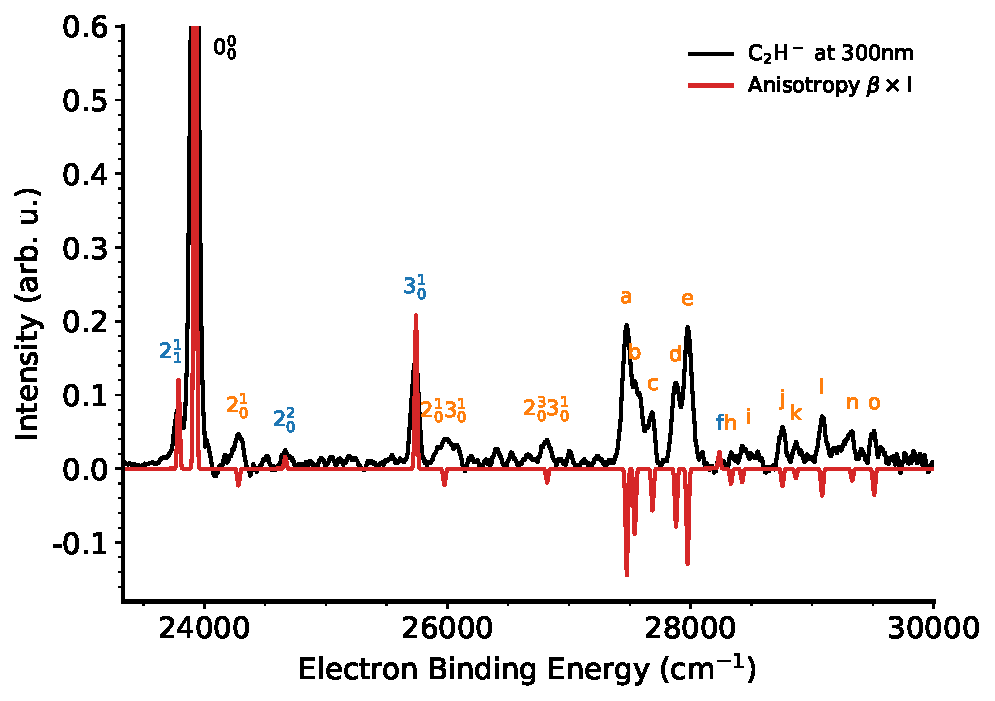
\includegraphics[width=0.6\textwidth]{figures/plotBeta.pdf}
	\caption{cat}
	\label{fig:beta}
\end{figure}

This result demonstrates how experimental anisotropies and calculated transition intensities can be used to help assign and understand vibronically coupled spectra. This is particularly useful in regions where there a large number of potential vibronic states, making definitive assignments based on energetics alone difficult.
%%%%%%%%%%%%%%%%%%%%%%%%%%%%%%%%%%%%%


 
\section{Conclusions} 

 
\section{Methods}
Details of the HR-PEI spectrometer are given in Refs~\onlinecite{cav07} and~\onlinecite{dev17}. CH$_2$CN$^-$ ions are produced by passing a 1:1 C$_2$H$_4$:N$_2$O gas mixture through a pulse valve, which then undergoes supersonic expansion into a high-voltage discharge. Negative ions are extracted, accelerated to 500~eV, and focussed into a novel gating, bunching, and re-referencing unit~\cite{ded01}. Anions are mass separated over a 2m time-of-flight region, with the ion of interest isolated by an electrostatic gate. The ion packet is crossed with a tuneable detachment laser beam, generated from a Sunlite EX optical parametric oscillator pumped by the third harmonic of a Continuum Powerlite 9010 Nd:YAG laser. The laser produces between 10-50mJ per pulse at 10Hz, depending on whether the idler or signal beam is used. The wavelength of the laser light is measured using a HighFinesse WS7 UV wavemeter.

A velocity-map imaging lens, a modified version of the original concept of Eppink and Parker, images the detached electrons to a 75mm diameter MCP/phosphor screen detector. Events are imaged by a 2014x2048 monochrome CCD camera (PCO 2000), with each frame transferred to a computer at a 10Hz repetition rate, and processed in real time to identify individual electron events. The electron positions are centroided to a sub-pixel accuracy, then written to a data file for subsequent analysis. The velocity-map image is centred and then circularized by an angular dependent-radial scaling determined by comparing adjacent radial slice intensity profiles~\cite{gas17}. An inverse Abel transformation of the VMI, based on the algorithm of Hansen and Law~\cite{han85,pya16}, returns a slice image of the 3D electron source distribution. Absolute energy calibration of the photoelectron spectra is achieved using published measurements of species, including O$^-$~\cite{cav07} and NO$_2^-$~\cite{law19}, that have been studied under similar conditions as used for the CH$_2$CN$^-$ measurements.

In standard operation, the energy distribution of the detached electrons is obtained by recording the velocity-mapped positions from photodetachment at a fixed wavelength. However the HR-PEI spectrometer may also be reconfigured into an electron counting mode, where the number of events per laser shot is recorded, while the detachment laser wavelength is varied.







%Hi~\cite{law17}

\begin{acknowledgement}
	This research was supported by the Australian Research Council Discovery
	Project Grants DP160102585 and DP190103151.  
\end{acknowledgement}

% Create the reference section using BibTeX: 
\bibliography{2022C2H.bib}

\end{document}
% ****** End of file apstemplate.tex ******